\section{Comparison to Sockets}\label{sec:comparison-to-sockets}
Since the aim of the API is to replace the existing BSD sockets API, a comparison between both APIs is important.
For this comparison, two implementations of a program which attempts a DNS lookup for a given domain name and connects
to first successful connection attempt, prioritising IPv6 addresses over IPv4 addresses.
See Appendix~\ref{ch:bsd-sockets-connection-code} for the sockets code and Appendix~\ref{ch:taps-connection-evaluation-code}
for the TAPS code.

\subsection{Latency Comparison}\label{subsec:latency-comparison}
Performance is important for network programming, and as discussed in Chapter~\ref{ch:analysis/requirements} the new
API should have performance similar to BSD sockets (sockets).
To have a fair comparision between the two API, the sockets version must also prioritise IPv6 addresses over IPv4
addresses, since the TAPS version does this internally.
Since a DNS lookup could have a large impact on the total latency, the domain tested is requested multiple times before
running the program under test.
See Appendix~\ref{ch:bash-script-for-latency-testing} for the script used to test the two programs.

\begin{figure}[h]
    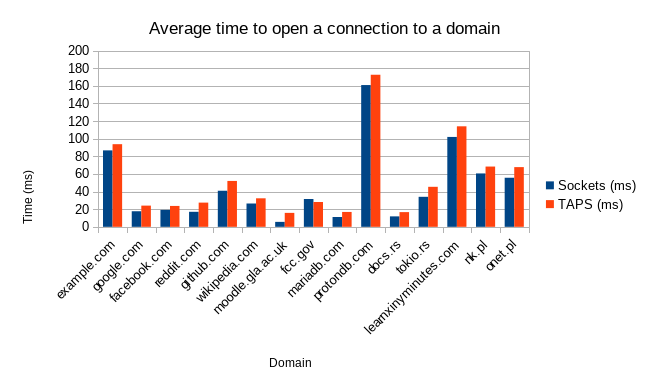
\includegraphics[width=\textwidth]{../data/avg_latency}
    \caption{A graph to show the average time over 10 attempts to connect to a range of domains.}
    \label{fig:latency}
\end{figure}

One style of network program is a short-lived program which only opens a single connection.
A program like this is useful for scripting and Unix Pipelines.
Figure~\ref{fig:latency} shows the time it takes to open a connection with both sockets and TAPS .

Figure~\ref{fig:latency} shows the TAPS version was slower for almost all domain tested when compared to the sockets
version.
Since the sockets version is single-threaded and not asynchronous, it doesn't need to set up a runtime for
\texttt{Future}s unlike the TAPS version.
In this particular test, the runtime had to be initialised ten times for each domain tested, leading to an overhead the
sockets version lacks.


%\subsection{Code Comparison}\label{subsec:lines-of-code-comparison}
%While lines of code is not a good metric to determine the quality of code, the substantial difference between the two
%implementations is worth discussing.
%Since sockets is a lower level library than TAPS, more code is required to do the same work as in TAPS .
%Opening a connection with the sockets API requires the following:
%\begin{itemize}
%    \item DNS lookup via \texttt{getaddrinfo}
%    \item Reorder DNS responses to prioritise IPv6 addresses
%    \item Open a socket
%    \item Connect to the remote server
%\end{itemize}
%The TAPS API does this all within \emph{Preconnection}'s \texttt{initiate} method.

%How good is your solution? How well did you solve the general problem, and what evidence do you have to support that?
%
%\section{Guidance}
%\begin{itemize}
%    \item
%        Ask specific questions that address the general problem.
%    \item
%        Answer them with precise evidence (graphs, numbers, statistical
%        analysis, qualitative analysis).
%    \item
%        Be fair and be scientific.
%    \item
%        The key thing is to show that you know how to evaluate your work, not
%        that your work is the most amazing product ever.
%\end{itemize}
%
%\section{Evidence}
%Make sure you present your evidence well. Use appropriate visualisations, reporting techniques and statistical analysis, as appropriate.
%
%If you visualise, follow the basic rules, as illustrated in Figure~\ref{fig:boxplot}:
%\begin{itemize}
%\item Label everything correctly (axis, title, units).
%\item Caption thoroughly.
%\item Reference in text.
%\item \textbf{Include appropriate display of uncertainty (e.g. error bars, Box plot)}
%\item Minimize clutter.
%\end{itemize}
%
%See the file \texttt{guide\_to\_visualising.pdf} for further information and guidance.
%
%\begin{figure}
%    \centering
%    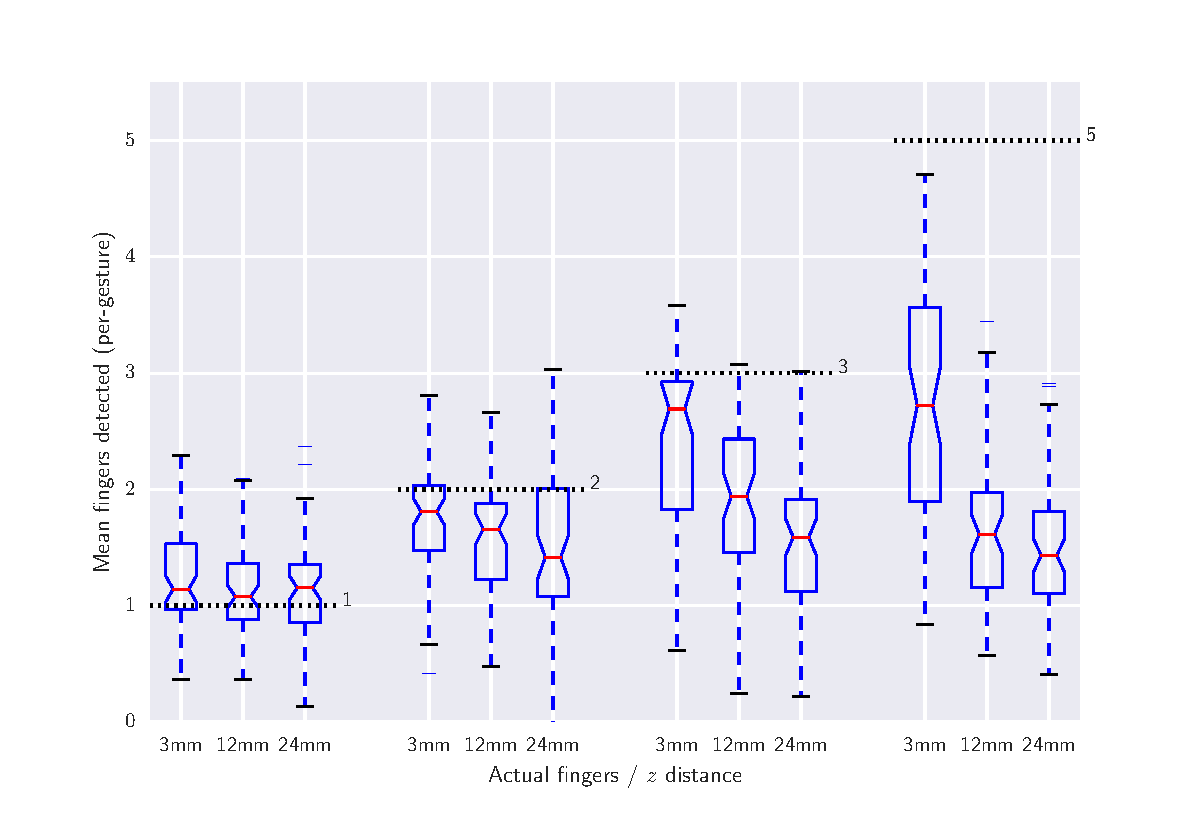
\includegraphics[width=1.0\linewidth]{images/boxplot_finger_distance.pdf}
%
%    \caption{Average number of fingers detected by the touch sensor at different heights above the surface, averaged over all gestures. Dashed lines indicate
%    the true number of fingers present. The Box plots include bootstrapped uncertainty notches for the median. It is clear that the device is biased toward
%    undercounting fingers, particularly at higher $z$ distances.
%    }
%
%    % use the notation fig:name to cross reference a figure
%    \label{fig:boxplot}
%\end{figure}
